\section{Experiments}
\label{sec:expe}

%\subsection{Methodology}
\label{sec:exp-methodo}

%This section briefly discusses our experimental setup for the evaluation of
%\Moca.

All our experiment were run on  machines from Grid5000 \emph{Edel} cluster
\footnote{A full hardware description is available online:\\
    \url{https://www.grid5000.fr/mediawiki/index.php/Grenoble:Hardware\#Edel}}.
    \DB{Do a table or something more visual}
These machines are composed of $2$ quad core \texttt{Intel Xeon E5520}
clocked at \SI{2.27}{GHz} with
\SI{24}{GB} of RAM. Hyper threading has been disabled during the experiment.
We deployed a \emph{Debian} \emph{Wheezy} environment running a Linux $3.2.41-2$.
To make the experiments reproducible, the environment and the trace files are
available
online~\footnote{Experiment traces and environments are available here:\\ \url{http://moais.imag.fr/membres/david.beniamine/experiments.html}}.

We present evaluation results for all the \NPB~\cite{Jin1999}. For
each benchmarks, we compare \Moca with the Pin instrumentation
used in Tabarnac~\cite{Beniamine15TABARNACRR}, one of our previous contribution. This instrumentation traps all the
memory accesses but keeps only tracks of the number of time each thread accesses to
each page, without any other information. Thus it does not require the management
of all the data structures necessary for \Moca.

Each point in each plot is the average of at least $30$ executions. Along with each point,
the error bars represent the standard deviation.
Except for the experiment about the influence of \Moca's parameters, on each
experiment, \Moca was run with it's default parameters: a wakeup interval of
\SI{0.5}{s} for the logging process and \SI{40}{ms} for the monitoring thread.

%\subsection{Experiments}
\subsection{Moca default parameters}
\label{sec:expe-param}

\begin{figure}[htb]
    \centering
    \begin{subfigure}{\linewidth}
        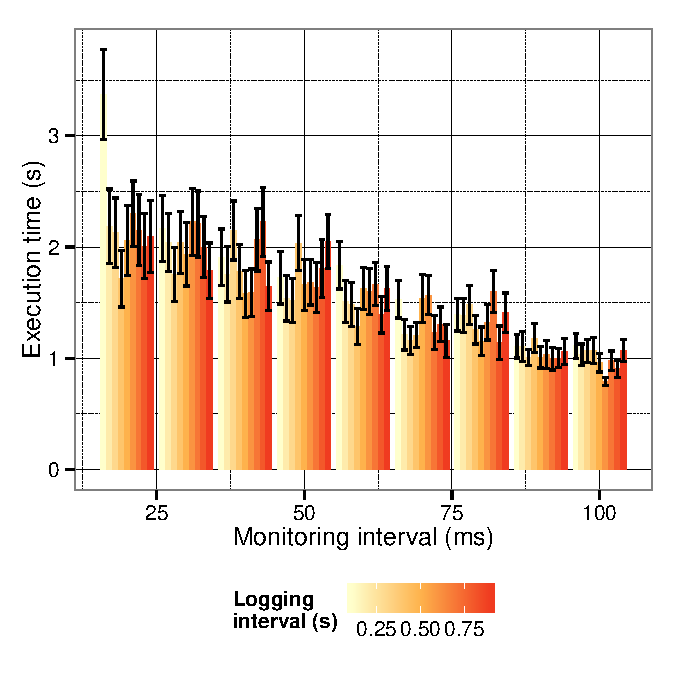
\includegraphics[width=\linewidth]{moca_param.pdf}
        \caption{Execution time.}
        \label{fig:param_time}
    \end{subfigure}

    \begin{subfigure}{\linewidth}
        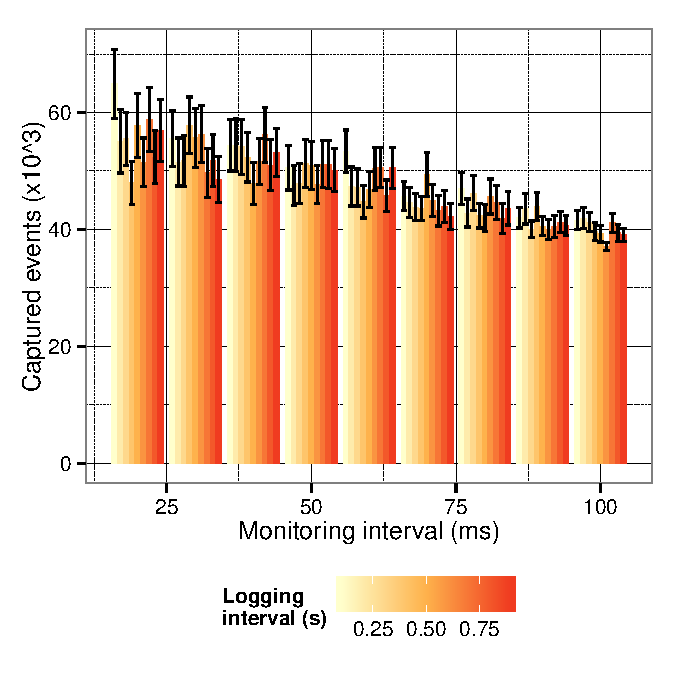
\includegraphics[width=\linewidth]{moca_param_events.pdf}
        \caption{Number of captured events.}
        \label{fig:param_evts}
    \end{subfigure}
    \caption{Influence of the wakeup intervals on \IS, class A.}
    \label{fig:param}
\end{figure}

Before comparing \Moca to existing tools, we need to evaluate the impact of
the wakeup intervals (logging daemon and monitor thread) on the trace
precision and on the overhead. To do so, we run the \IS benchmark instrumented by \Moca with
a wakeup interval ranging from \SI{0.1}{s} to  \SI{0.9}{s} for the logging daemon and from \SI{20}{ms} to
\SI{100}{ms} for the monitoring thread. For each run, we measure \IS execution time and the number of
accesses captured. We have chosen \IS for this evaluation as it is one of the memory intensive \NPB,
quick experiments with other ones confirmed these results.

We can see on the \fig{fig:param_time} that performances seem too decrease linearly
as the monitoring interval decreases. A closer examination reveals that results
suffer from a high variability under \SI{40}{ms}. 
In addition, the \fig{fig:param_evts} shows
that, at \SI{40}{ms}, \Moca can capture a significant number of events, not significantly improved
\GH{Sur les figures, je vois plutôt 60ms et 50ms repectivement comme intervalles interessants\ldots}
\DB{Les ecarts se sont resserés avec le nombre de runs \ldots}
by lower wakeup intervals. Having chosen this interval of \SI{40}{ms} seconds for the monitoring thread,
we found out that waking up the logging process every \SI{0.4}{s} gave a sufficient reactivity to store
all the collected events.
These two values have been chosen as default values in \Moca.

\subsection{Comparison with existing tools}
\label{sec:expe-ovh}
\DB{New: MemProf, Tabarnac, Moca, Moca + Pin}
To evaluate \Moca fairly, we have chosen a tool that also provides a superset of
all the memory accesses (see table \ref{tab:tools-comp}). Therefore, we have chosen the Pin
instrumentation used in Tabarnac. All the experiment presented here have been run on
all the \NPB on class A.
\DB{See new figure, maybe log scale ?}

\begin{figure}[htb]
    \centering
    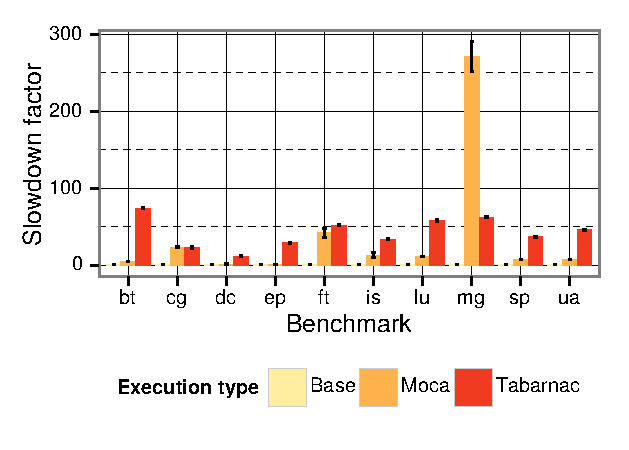
\includegraphics[width=\linewidth]{moca_overhead_nas.pdf}
    \caption{Slowdown of \Moca on the \NPB compared to
    Tabarnac.}
    \label{fig:ovh}
\end{figure}

\fig{fig:ovh} shows the slowdown of each benchmark, respectively instrumented with \Moca and Tabarnac and compared to
an uninstrumented execution. We can classify these results into three groups of
applications:  for \BT, \DC, \EP, \IS, \LU, \SP and \UA, \Moca is
significantly faster than Tabarnac. This set of benchmarks is interesting as it is made of varied application profiles.
Indeed, if \EP is mostly doing parallel computation with only a few number of
memory accesses, \IS is memory intensive with a random memory access pattern and
\BT, \LU as well as \SP are pseudo applications doing a significant usage of memory.
And while \DC and \UA are categorised as \emph{unstructured computation,
parallel I/O and data movement} by the \NPB website
\footnote{\url{http://www.nas.nasa.gov/publications/npb.html}}, their interaction with memory seems noticeable.
The second group only contains memory oriented benchmarks (\CG and \FT). For this group,
\GH{C'est plutôt équilibré calcul / accès mémoire, non ?}
\DB{Boaf la description CG dit ``irregular memory accesses and communication''
et \FT ``all to all communications}
\Moca is as good as Tabarnac or a bit faster, probably because the balance between computations and memory accesses hides the overhead of the instrumentation.
Finally for \MG, \Moca is
significantly slower than Tabarnac. This benchmark seems to be a pathological
case were the execution time with \Moca has a lot a variability. Actually, in this benchmark, the quantity of pages accessed is huge and exceeds the size
allocated for \Moca data structures. This results in the triggering of \Moca routines that recycle parts of the recent accesses to accept new ones.
We suspect that this is the cause if its bad beahavior.
\DB{Je sais pas vraiment comment présenter les resultats de \MG, c'est mauvais
et variable (sur une centaine de runs ici, la moitié sont très lent et l'autre
moitié plus proche de tabarnac)}
\GH{Et les exec avec plus de mémoire dans le module ?}
\DB{Ca a merdé ya des soucis avec la migration OAR vers postgresql}
Overall, these experiments show that \Moca is significantly faster than a typical tool based on binary instrumentation
for a majority of benchmarks, and at least as good for most of the others.

\begin{figure}[htb]
    \centering
    \begin{subfigure}{\linewidth}
        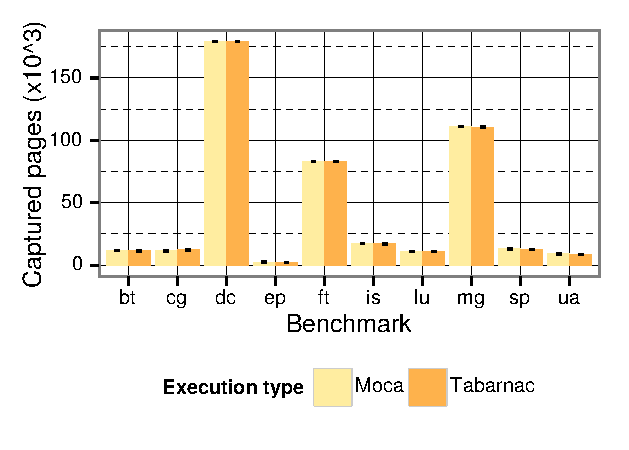
\includegraphics[width=\linewidth]{moca_pages_nas.pdf}
        \caption{Number of pages.}
        \label{fig:pages}
    \end{subfigure}
    \begin{subfigure}{\linewidth}
        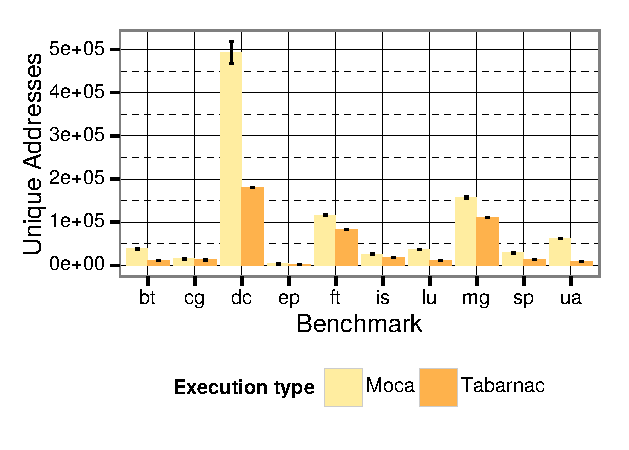
\includegraphics[width=\linewidth]{moca_addresses_nas.pdf}
        \caption{Number of unique addresses.}
        \label{fig:addr}
    \end{subfigure}
    \caption{Number of pages and unique addresses captured by \Moca and Tabarnac
    on the \NPB.}
    \label{fig:pages-addr}
\end{figure}

Then, we have compared the number of pages and unique addresses captured by \Moca
and Tabarnac during the previous experiment. As expected and as we can see in figure
\fig{fig:pages}, both methods capture the exact same number of
pages, which is the superset of all the memory accesses. Furthermore,
\fig{fig:addr} shows that \Moca also provides a more precise trace than Tabarnac
regarding the number of unique addresses collected. This can be explained by the 
radically different designs of the two tools. While \Moca keeps track of all
the pages accessed during the execution, it also stores, for each triggered page fault, the
exact address of the memory access. On the contrary, to keep the overhead small,
a tool like Tabarnac has to work at a coarser granularity: it only counts the number
of accesses performed by the application for each page address. The result is that Tabarnac
collects space data with the precision of the page (4096 bytes) while \Moca collects them with
the precision of the byte.

\subsection{Summary}
\label{sec:expe-cncl}

We have tested \Moca with various applications and using several parameters.
Our experiments, show that \Moca has a good behavior for a wide range of parameter and
helped us defining their default values. Our experiments also show that, with these
parameters, \Moca is at worst as slow as comparable tools and in most 
cases faster. Moreover, \Moca provides more precise traces than comparable tools.
It is noteworthy that \Moca is the only tool able to provide a detailed trace with temporal,
spacial and sharing information while providing guarantees on the information
% \GH{Tu ne parles vraiment de sharing qu'ici !!}
% \DB{Dans la Table I de design aussi, j'ai modifié un paragraphe pour insister
% dessus}
lost during the sampling.
